
%Inicio 
\chapter{Listas Encadeadas}
\chaplabel{linkedlists}

\index{linked list}%
Neste capítulo, continuamos a estudar implementações da interface # List #, 
desta vez utilizando estruturas de dados baseadas em ponteiro em vez de 
arrays. As estruturas neste capítulo são constituídas por nós que contêm 
os itens da lista. Usando referências (ponteiros), os nós são encadeados 
em uma sequência. Primeiro, estudamos listas simplesmente encadeadas, 
que podem implementar as operações de uma # Stack # e de uma # Queue # (FIFO)   
em tempo constante por operação e, em seguida, passamos para listas duplamente 
encadeadas, que podem implementar operações de # Deque #  em tempo constante.

As listas encadeadas têm vantagens e desvantagens quando comparadas com implementações 
baseadas em array da interface # List #. A principal desvantagem é que perdemos 
a capacidade de acessar qualquer elemento usando #get(i) # ou #set(i,x) # 
em tempo constante. Em vez disso, temos de percorrer a lista, um elemento de 
cada vez, até chegar ao #i#-ésimo elemento. A principal vantagem é que elas são 
mais dinâmicas: dada uma referência a qualquer nó de lista  # u #, podemos apagar 
# u # ou inserir um nó adjacente a # u # em tempo constante. Isso é verdade, 
não importa onde # u # esteja na lista.

\section{#SLList#: Uma Lista Simplesmente Encadeada}
\seclabel{sllist}

\index{SLList@#SLList#}%
\index{linked list!singly-}%
\index{singly-linked list}%
Uma # SLList # (lista simplesmente encadeada) é uma sequência de \textit{Nó}s. Cada nó 
# u # armazena um valor de dados # u.x # e uma referência # u.next # para o 
próximo nó na sequência. Para o último nó # w # na sequência, $ # w.next # = # null # $

% TODO: Remove constructors from SLList.Node
\javaimport{ods/SLList.Node}
\cppimport{ods/SLList.Node}

Para eficiência, um # SLList # usa as variáveis # head # e # tail # para 
manter o registro do primeiro e do último nó na sequência, bem como um número 
inteiro # n # para acompanhar o tamanho da sequência:
\codeimport{ods/SLList.head.tail.n}
Uma sequência de operações em um # Stack # e uma # Queue #  em um # SLList # é 
ilustrada na \figref{sllist}.

\begin{figure}
  \begin{center}
    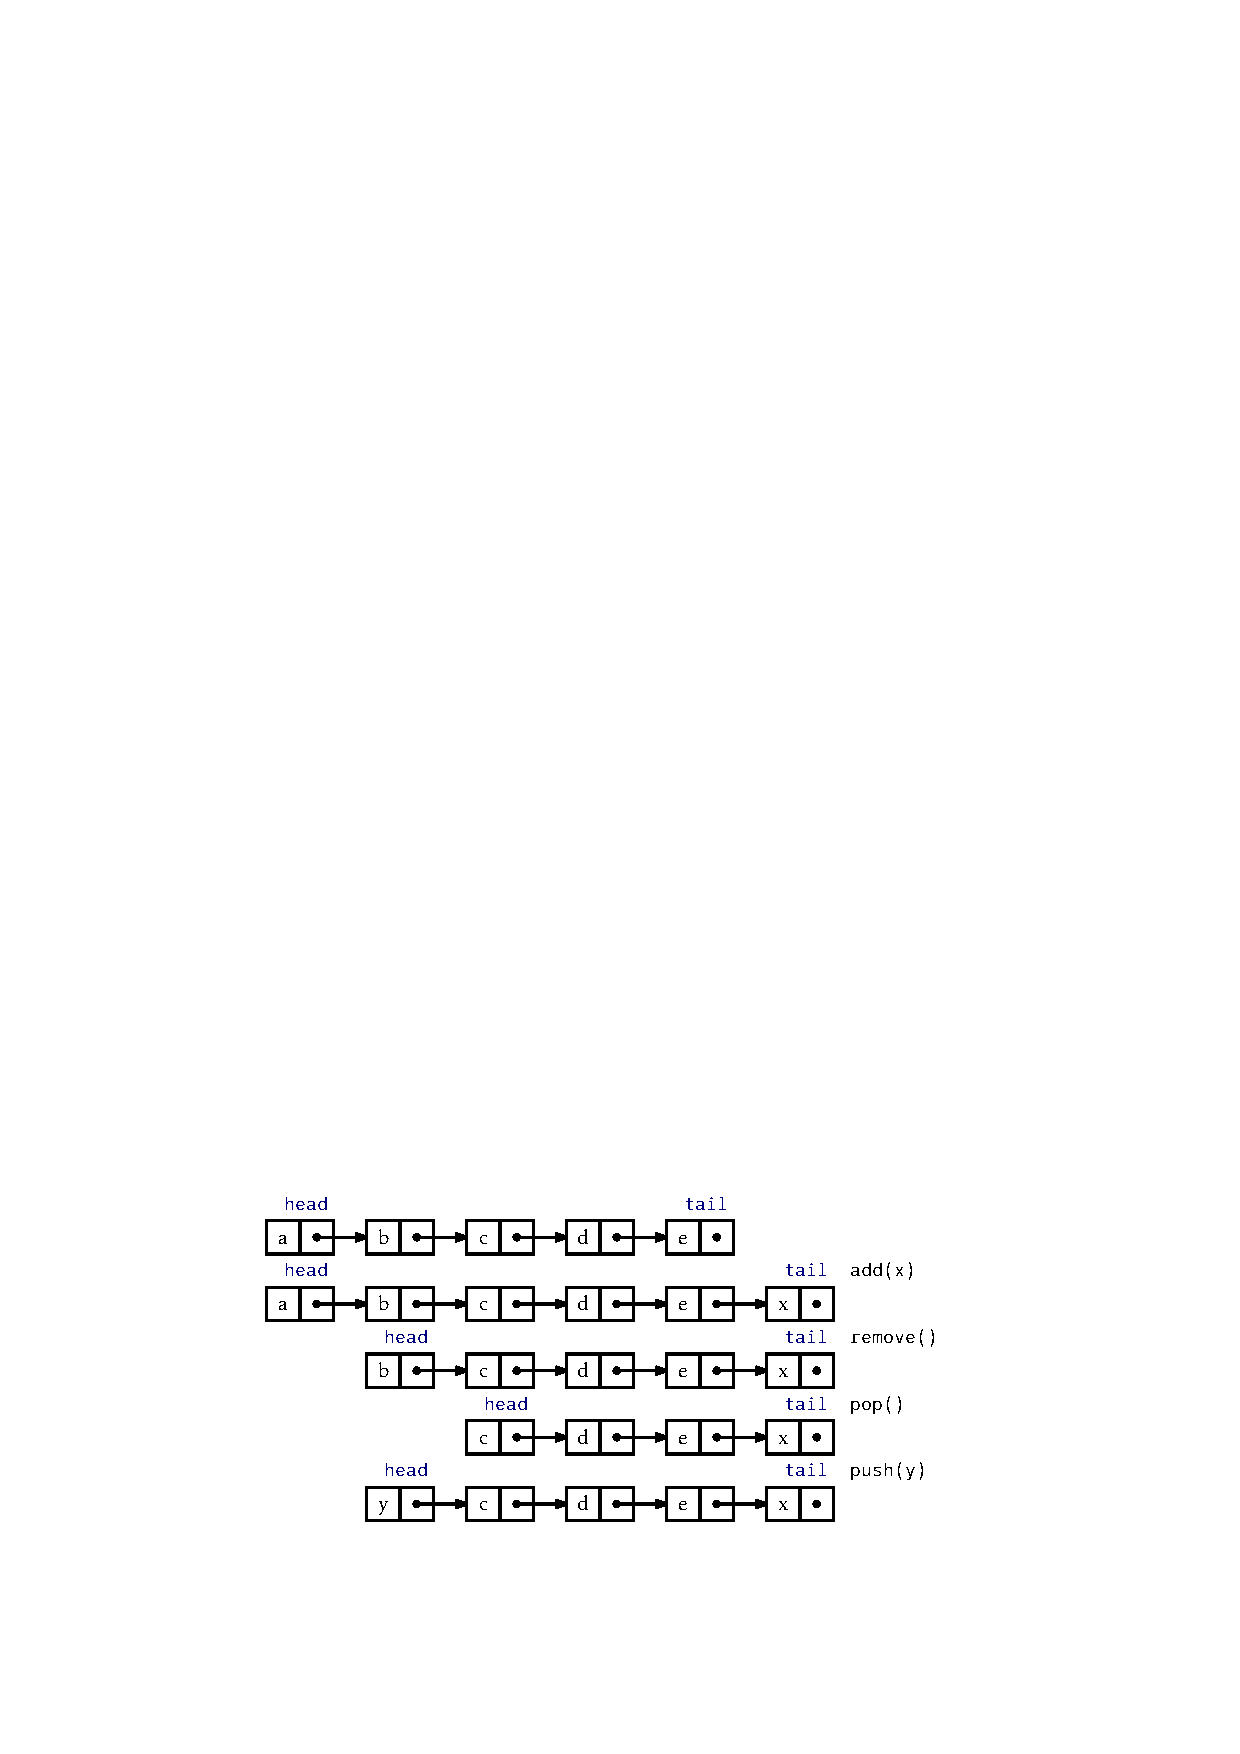
\includegraphics[width=\ScaleIfNeeded]{figs/sllist}
  \end{center}
  \caption[Uma sequência de operações de fila e pilha em uma SLList] {Uma sequência de operações de # Queue # 
  	(#add(x)# e #remove()#) e de #Stack# (#push(x)# e #pop()#) em uma #SLList#.}
  \figlabel{sllist}
\end{figure}

Uma #SLList# pode implementar eficientemente as operações #push()# e #pop()# 
de uma #Stack#, adicionando e removendo elementos na cabeça da sequência. 
A operação #push()# simplesmente cria um novo nó #u# com valor de dados #x#, 
define #u.next# no cabeçalho antigo da lista e torna #u# o novo cabeçalho 
da lista. Finalmente, ele incrementa #n#, uma vez que o tamanho da #SLList# 
aumentou em um:

\codeimport{ods/SLList.push(x)}

A operação #pop()#, depois de verificar que a #SLList# não está vazia, 
remove a cabeça definindo $#head=head.next#$ e decrementando #n#. 
Um caso especial ocorre quando o último elemento está sendo removido, 
caso em que #tail# é definido como #null#:

\codeimport{ods/SLList.pop()}

Claramente, as operações #push(x)# e #pop()# são executadas em tempo $O(1)$.

\subsection{Operações de Fila}

Uma # SLList # também pode implementar as operações de fila FIFO, #add(x)# e 
#remove()#, em tempo constante. As remoções são feitas a partir da cabeça 
da lista e são idênticas à operação #pop()#:

\codeimport{ods/SLList.remove()}

Adições, por outro lado, são feitas no final da lista. Na maioria dos casos, isso é 
feito definindo $#tail.next#=#u#$, onde #u# é o nó recém-criado que contém #x#. 
No entanto, um caso especial ocorre quando $#n#=0$, caso em que $#tail#=#head#=#null#$. 
Nesse caso, tanto #tail# como #head# são definidos como #u#.

\codeimport{ods/SLList.add(x)}

Claramente, ambos #add (x) # e #remove () # levam tempo constante.

\subsection{Resumo}

O seguinte teorema resume o desempenho de uma #SLList#:

\begin{thm}\thmlabel{sllist}
  Uma #SLList# implementa a interface para #Stack# e (FIFO) #Queue#. 
  As operações #push(x)#, #pop()#, #add(x)# e #remove()# são executadas 
  em um tempo $O(1)$ por operação.
\end{thm}
%fim eu
%Inicio Pedro

Uma #SLList# quase implementa o conjunto completo de operações de uma #Deque#.
A única operação que falta é a remoção da cauda de uma #SLList#.
Remover a cauda de uma #SLList# é difícil porque requer a atualização do valor da #tail# para que ele aponte para o nó #w# que precede #tail# na # SLList #; este é o nó #w# tal que $#w.next#=#tail#$. Infelizmente, a única maneira de chegar ao #w# é atravessar a #SLList# começando em #head# e tomando $#n#-2$ passos.

\section{#DLList#: Uma lista duplamente encadeada}
\seclabel{dllist}

\index{DLList@#DLList#}%
\index{doubly-linked list}%
\index{linked list!doubly-}%
A #DLList# (lista duplamente encadeada) é muito semelhante a uma #SLList#, exceto que cada nó #u# em uma #DLList# tem referências tanto ao nó #u.next# que o sucede, quanto ao nó #u.prev# que o precede.

\javaimport{ods/DLList.Node}
\cppimport{ods/DLList.Node}

Ao implementar uma #SLList#, vimos que sempre havia vários casos especiais para se preocupar. Por exemplo, remover o último elemento ou adicionar um elemento vazio a uma #SLList# requer cuidado para garantir que #head# e #tail# sejam atualizados corretamente. Numa #DLList#, o número destes casos especiais aumenta consideravelmente. Talvez a maneira mais limpa de cuidar de todos esses casos especiais numa #DLList# é introduzir um nó #dummy#.
\index{dummy node}%
Este é um nó que não contém quaisquer dados, mas age como um espaço reservado para que não haja nós especiais; cada nó tem um #next# e um #prev#, com o #dummy# agindo como o nó que sucede o último nó na lista e que precede o primeiro nó na lista. Desta forma, os nós da lista são (duplamente) ligados em um ciclo, como ilustrado na \figref{dllist}.


\begin{figure}
	\begin{center}
		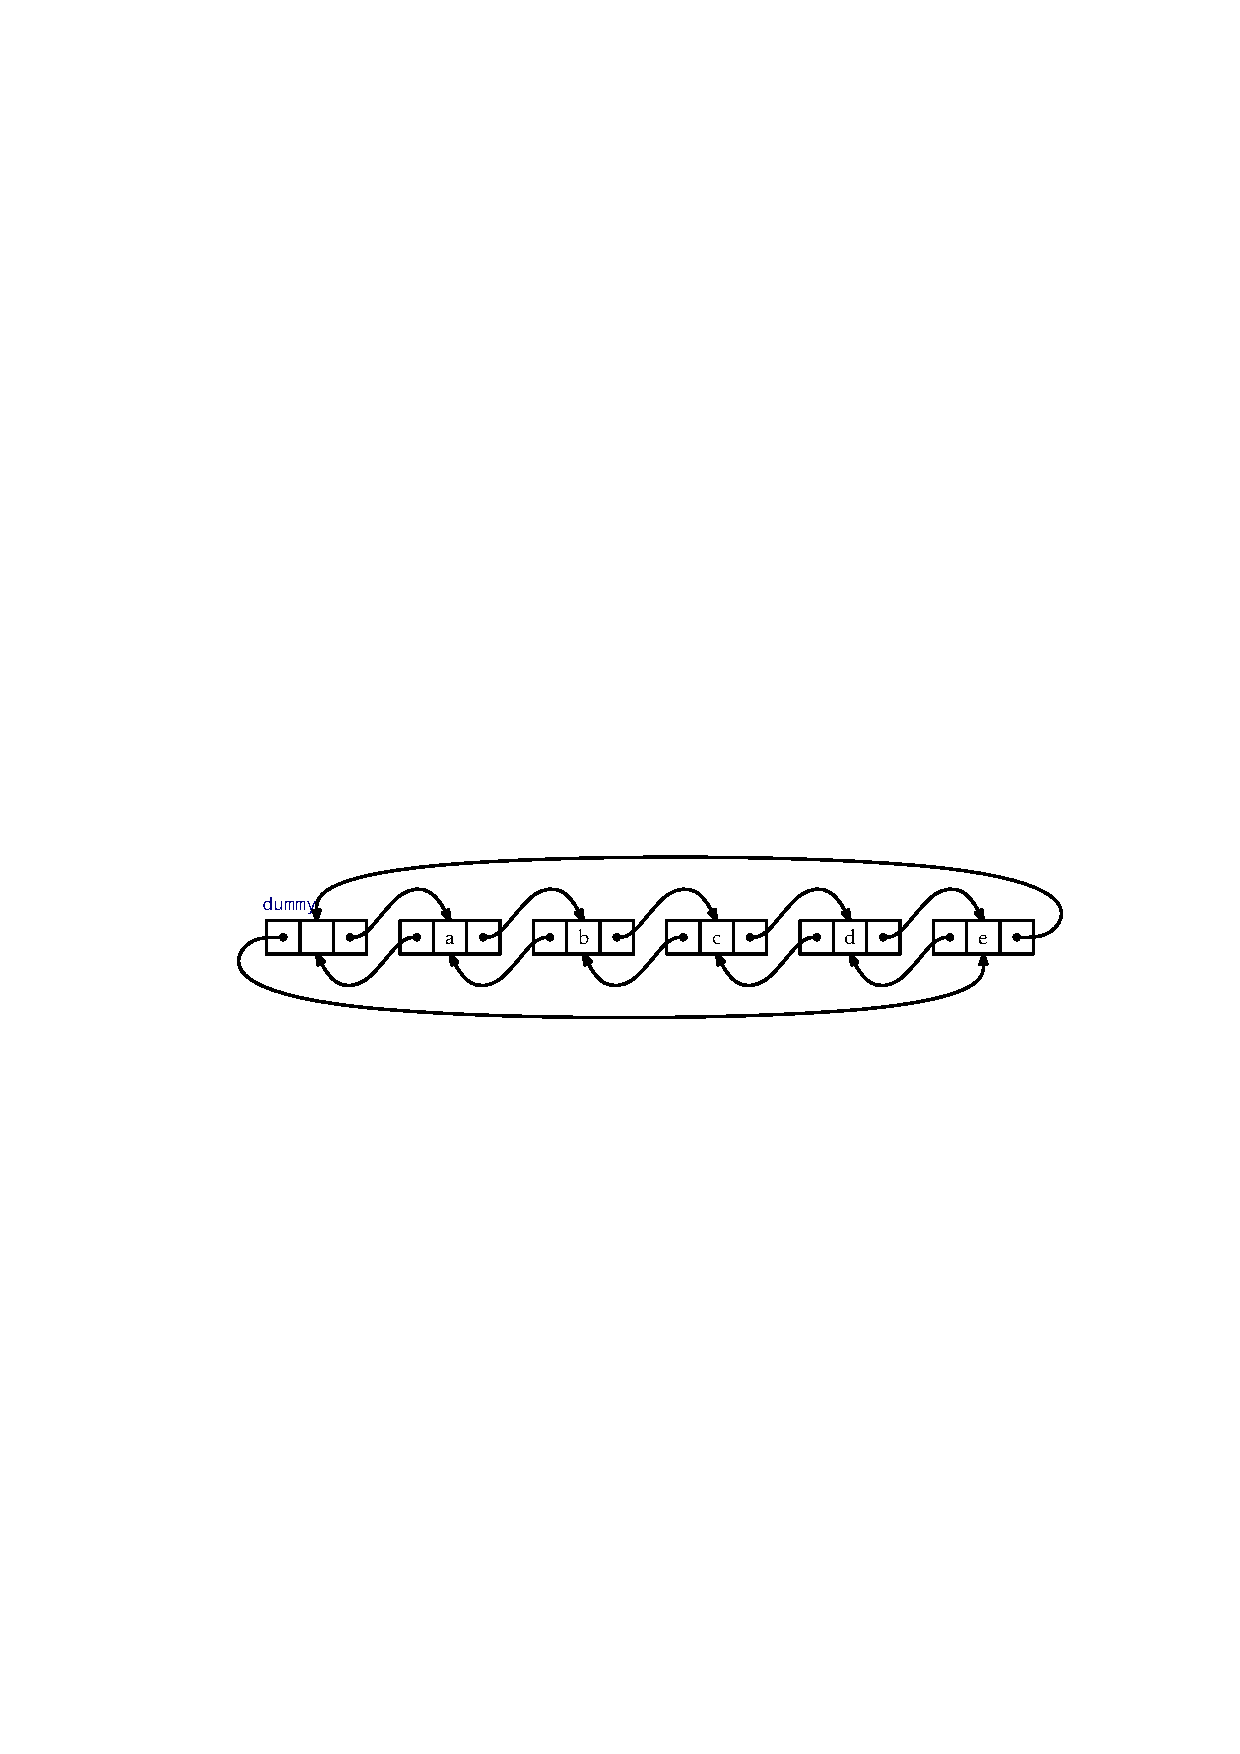
\includegraphics[width=\ScaleIfNeeded]{figs/dllist2}
	\end{center}
	\caption[A DLList]{Uma #DLList# contendo a,b,c,d,e.}
	\figlabel{dllist}
\end{figure}


%TODO: Remove constructors from class Node

\codeimport{ods/DLList.n.dummy.DLList()}

Encontrar um nó com um índice específico em uma #DLList# é fácil. Podemos começar na cabeça da lista (#dummy.next#) e trabalhar para a frente, ou começar no final da lista (#dummy.prev#) e trabalhar para trás.
Isso nos permite alcançar o #i#-ésimo nó em $O(1+\min\{#i#,#n#-#i#\})$:

\codeimport{ods/DLList.getNode(i)}

As operações #get(i)# e #set(i,x)# agora também são fáceis. Em primeiro lugar, localizamos o #i#-ésimo nó e depois obtemos(get) ou definimos(set) seu valor #x#:

\codeimport{ods/DLList.get(i).set(i,x)}

O tempo de execução dessas operações é dominado pelo tempo que leva para encontrar o #i#-ésimo nó, sendo assim, $O(1+\min\{#i#,#n#-#i#\})$.

\subsection{Adicionando e Removendo}

Se tivermos uma referência a um nó #w# numa #DLList# e quisermos inserir um nó #u# antes de #w#, então isto é apenas uma questão de definir $#u.next#=#w#$, $#u.prev#=#w.prev#$ e, em seguida, ajustar #u.prev.next# e #u.next.prev#. (Ver \figref{dllist-addbefore}.)
Graças ao nó dummy, não há necessidade de se preocupar se #w.prev# ou #w.next# não existam.

\codeimport{ods/DLList.addBefore(w,x)}

\begin{figure}
	\begin{center}
		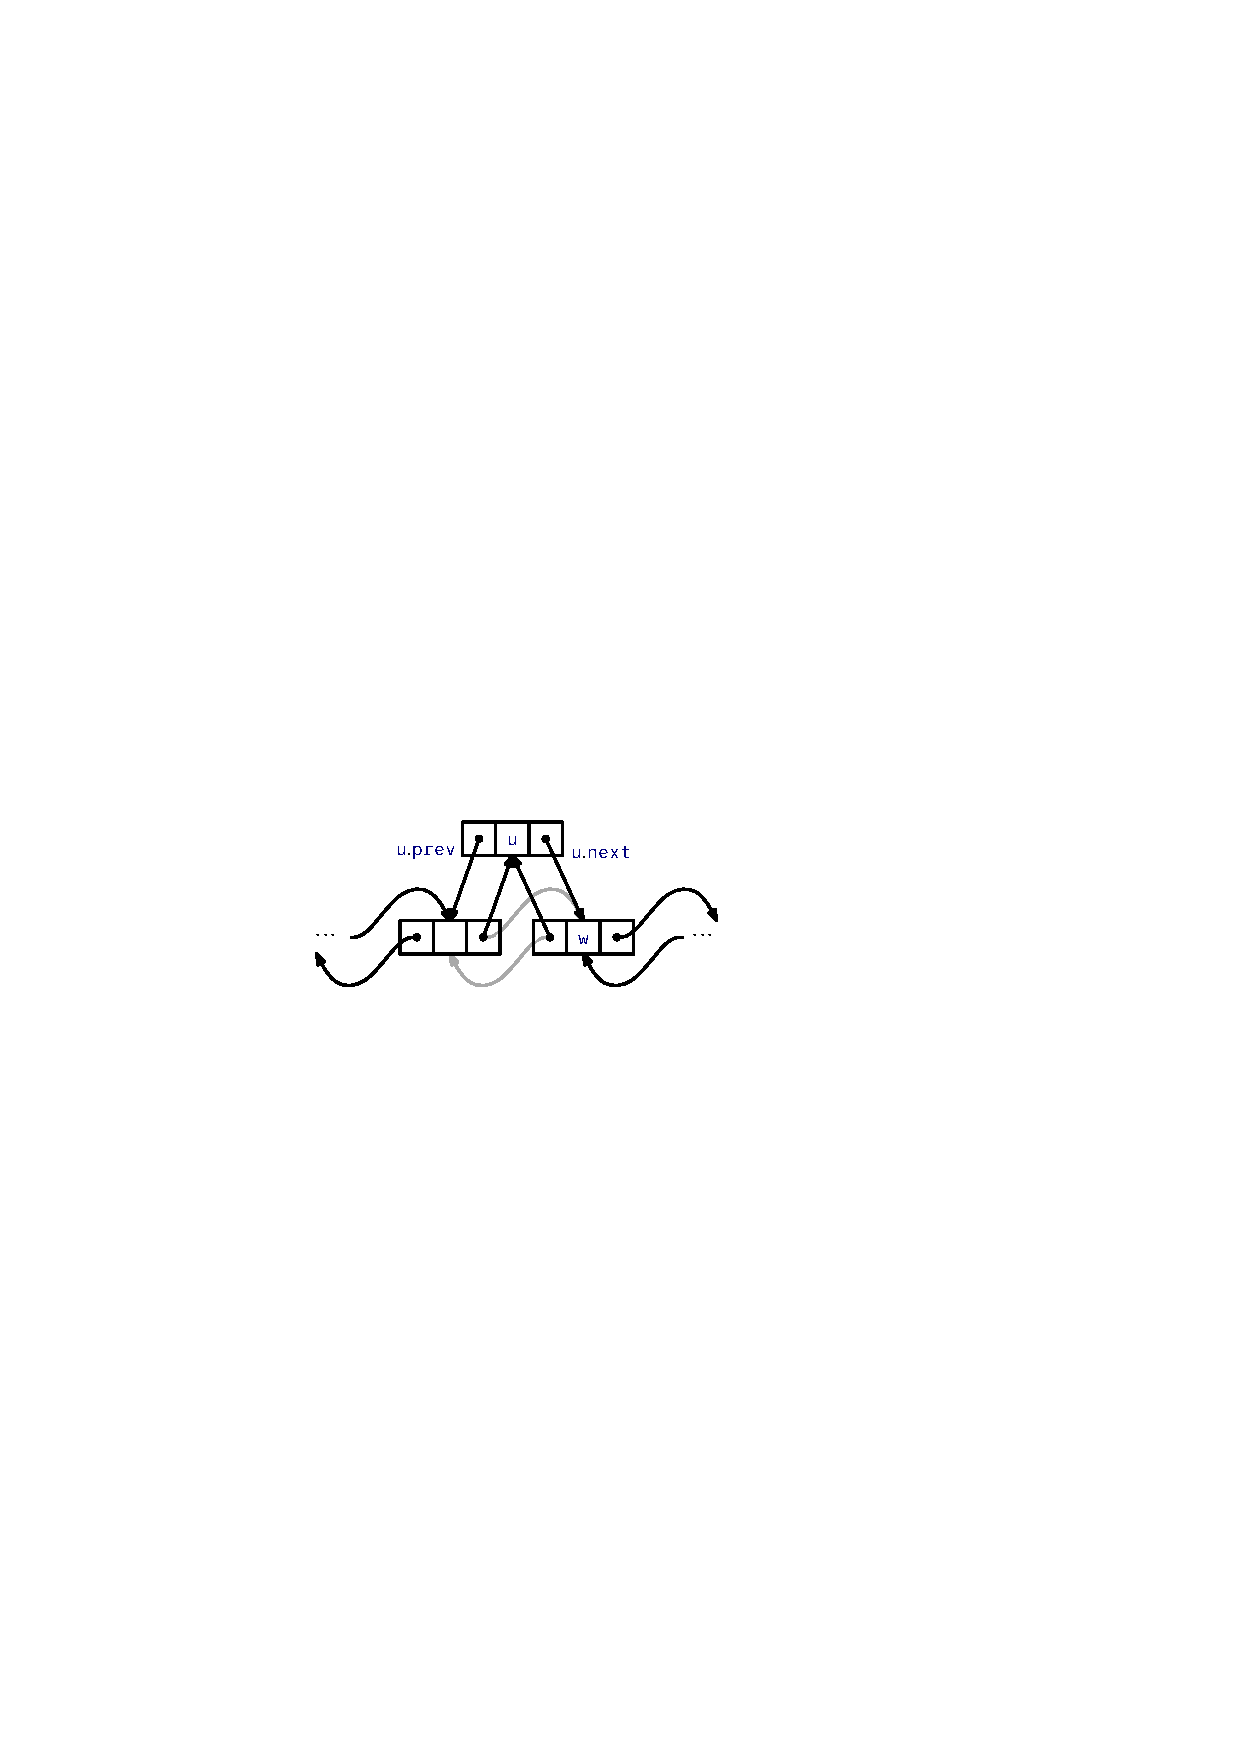
\includegraphics[scale=0.90909]{figs/dllist-addbefore}
	\end{center}
	\caption[Adicionando a DLList]{Adicionando o nó #u# antes do nó #w# em uma #DLList#.}
	\figlabel{dllist-addbefore}
\end{figure}

Dessa forma, a operação de lista #add(i,x)# se torna trivial para implementar. Encontramos o #i#-ésimo nó na #DLList# e inserimos um novo nó #u# que contém #x# imediatamente antes dele.

\codeimport{ods/DLList.add(i,x)}

A única parte não constante do tempo de execução de #add(i,x)# é o tempo necessário para encontrar o #i#-ésimo nó (usando #getNode(i)#). Assim, #add(i,x)# é executado em $O(1+\min\{#i#, #n#-#i#\})$.

Remover um nó #w# da #DLList# é fácil. Nós só precisamos ajustar os ponteiros em #w.next# e #w.prev# para que eles pulem #w#. Novamente, o uso do nó dummy elimina a necessidade de considerar quaisquer casos especiais:
%Fim Pedro
%Inicio Matheus
\codeimport{ods/DLList.remove(w)}

Agora a operação #remove(i)# é trivial. Achamos o nó com índice #i# e removemos:

\codeimport{ods/DLList.remove(i)}

Novamente, a única parte cara dessa operação é achar o #i#-ésimo nó
usando #getNode(i)#, então #remove(i)# roda em $O(1+\min\{#i#, #n#-#i#\})$.

\subsection{Resumo}

O seguinte teorema resume o desempenho de uma #DLList#:

\begin{thm}\thmlabel{dllist}
	A #DLList# implementa a interface de uma #Lista#.  Na implementação,
	as operações #get(i)#, #set(i,x)#, #add(i,x)# e #remove(i)# executam
	em $O(1+\min\{#i#,#n#-#i#\})$ por operação.
\end{thm}

Vale notar que, se ignorarmos o custo da operação #getNode(i)#, 
então todas as operações da #DLList# levam tempo constante.
Portanto, a única parte cara das operações na #DLList# é achar
o nó relevante.  Uma vez tenhamos o nó relevante, adicionar, remover,
ou acessar os dados no nó leva tempo constante.

Isso contrasta claramente com as implementações da #Lista# baseada em array do
\chapref{arrays}; nessas implementações, o item relevante no array
pode ser encontrado com tempo constante. Entretanto, adicionar ou remover requer
uma mudança de elementos no array e, em geral, leva um tempo não constante.

Por essa razão, as estruturas de lista encadeadas são bem adequadas para aplicações em que 
as referências a nós de lista podem ser obtidas por meios externos.
\javaonly{Um exemplo disso é #LinkedHashSet# estrutura de dados encontrada no Framework
	Java Collections, na qual uma série de itens são guardados em
	listas duplamente encadeadas e os nós das listas duplamente encadeadas são guardadas
	na tabela de hash (discutida no \chapref{hashing}).  Quando elementos
	são removidos de uma #LinkedHashSet#, a tabela de hash é usada para encontrar a
	lista de nós relevantes em tempo constante e então a lista de nós é deletada
	(também em tempo constante).}
\cpponly{Por exemplo, ponteiros para os nós de uma lista encadeada podem ser
	guardados em uma #USet#.  Então, para remover um item #x# de uma lista encadeada,
	o nó que contém #x# pode ser rapidamente encontrado usando #Uset# e
	o nó pode ser removido da lista em tempo constante.}

\section{#SEList#: Uma Lista Encadeada Eficiente em Espaço}
\seclabel{selist}

\index{SEList@#SEList#}%
\index{linked list!space-efficient}%
Uma das desvantagens das listas encadeadas (além do tempo que leva para acessar
elementos que estão no final da lista) é o seu uso de espaço.  Cada nó
na #DLList# requer duas referências adicionais para o próximo nó
e o anterior na lista.  Dois desses campos no nó #Node# são dedicados
a manter a lista, e só um dos campos serve para armazenar dados!

Uma #SEList# (lista eficiente em espaço) reduz o desperdício de espaço usando
uma ideia simples: em vez de guardar os elementos individualmente numa #DLList#,
guardamos um bloco (array) contendo vários itens. Mais precisamente, a
#SEList# é parametrizada pelo \emph{tamanho do bloco} #b#. Cada nó individual
em uma #SEList# guarda um bloco que suporta até #b+1# elementos.

Por razões que ficarão claras mais à frente, será útil se pudermos fazer 
operações do #Deque# em cada bloco.  A estrutura de dados que escolhemos
para isso é a #BDeque# (bounded deque),
\index{BDeque@#BDeque#}%
\index{bounded deque}%
\index{deque!bounded}%
derivada da #ArrayDeque#,
estrutura descrita na \secref{arraydeque}.  O #BDeque# se diferencia do
#ArrayDeque# numa pequena coisa: quando um novo #BDeque# é criado, o tamanho
do array de suporte #a# é fixado em #b+1# e nunca cresce ou encolhe.
A propriedade importante do #BDeque# é que ele permite adição e remoção
de elementos por qualquer dos lados em tempo constante. Isso
será útil quando elementos forem trocados de um bloco para outro.

\javaimport{ods/SEList.BDeque} 
\cppimport{ods/SEList.BDeque} 

\notpcode{
	Uma #SEList# é então uma lista duplamente encadeada de blocos:
} % notpcode
\javaimport{ods/SEList.Node}
\cppimport{ods/SEList.Node}
\javaimport{ods/SEList.n.dummy}
\cppimport{ods/SEList.n.dummy}

\pcodeonly{
	Uma #SEList# é só uma lista duplamente encadeada de blocos. Além dos ponteiros #next# e #prev# , cada nó #u# em uma #SEList# contém um #BDeque#, #u.d#.
}

\subsection{Requisitos de Espaço}
%Fim Matheus
%Inicio Lucas
Uma #SEList# coloca restrições rígidas sobre o número de elementos em um bloco:
a menos que um bloco seja o último bloco, então esse bloco contém 
pelo menos $#b#-1$ e no máximo $#b#+1$ elementos. Isto significa
que, se um #SEList# contém #n# elementos, então ele tem no máximo
\[
#n#/(#b#-1) + 1 = O(#n#/#b#)
\]
blocos. A #BDeque# para cada bloco contém um array de comprimento $#b#+1$
mas, para cada bloco exceto o último, no máximo uma quantidade constante de
espaço é desperdiçada nesse array. A memória restante usada por um bloco também
é constante. Isso significa que o espaço perdido em uma #SEList# é apenas
$O(#b#+#n#/#b#)$. Ao escolher um valor de #b# dentro de um fator constante 
$\sqrt{#n#}$, podemos fazer o overhead de espaço de uma SEList se aproximar 
do limite inferior $\sqrt{#n#}$ dado na \secref{rootishspaceusage}.

\subsection{Encontrando Elementos }

O primeiro desafio que encontramos em uma #SEList# é encontrar o item da lista
com um dado index #i#.  Note que a localização do elemento é constituída por 
duas partes: 
\begin{enumerate}
	\item O nó #u# que contém o bloco que contém o elemento
	com o index #i#; e
	\item o index #j# do elemento dentro do bloco.
\end{enumerate}

\javaimport{ods/SEList.Location}
\cppimport{ods/SEList.Location}

Para encontrar o bloco que contém um determinado elemento, procedemos da mesma
maneira que em uma #DLList#. Ou começamos pela frente da lista se deslocando 
para frente, ou por trás da lista se deslocando para trás até chegar ao nó 
que queremos. A única diferença é que, cada vez que passamos de um nó para o 
próximo, nós pulamos um bloco inteiro de elementos.

\pcodeimport{ods/SEList.get_location(i)}
\javaimport{ods/SEList.getLocation(i)}
\cppimport{ods/SEList.getLocation(i,ell)}

Lembre-se que, com exceção de no máximo um bloco, cada bloco contém pelo
menos $#b#-1$ elementos, de modo que cada etapa em nossa pesquisa nos
deixa $#b#-1$ elementos mais próximos do elemento procurado. Se nós
estamos procurando para a frente, isto significa que atingimos o nó 
procurado após $O(1+#i#/#b#)$ passos. Se buscarmos para trás, então 
alcançamos o nó procurado após $O(1+(#n#-#i#)/#b#)$ passos. O algoritmo 
leva a menor dessas duas quantidades dependendo do valor de #i#, então o 
tempo para localizar o item com o índice #i# é $O(1+\min\{#i#,#n#-#i#\}/#b#)$.

Uma vez que saibamos como localizar o item com o índice #i#, as operações
#get(i)# e #set(i,x)# traduzem-se em obter ou definir um determinado
índice no bloco correto:

\codeimport{ods/SEList.get(i).set(i,x)}

Os tempos de execução destas operações são dominados pelo tempo que leva
para localizar o item, então eles também são executados no tempo
$O(1+\min\{#i#,#n#-#i#\}/#b#)$.

\subsection{Adicionando um Elemento}

Adicionar elementos em uma #SEList# é um pouco mais complicado. Antes de
considerar o caso geral, consideramos a operação mais fácil, #add(x)#,
na qual #x# é adicionado ao final da lista. Se o último bloco estiver cheio
(ou não existir porque ainda não tem blocos), então nós primeiro
alocamos um novo bloco e o anexamos à lista de blocos. Agora que
temos certeza de que o último bloco existe e não está cheio, anexamos #x#
no último bloco.

\cppimport{ods/SEList.add(x)}
\javaimport{ods/SEList.add(x)}
\pcodeimport{ods/SEList.append(x)}

As coisas ficam mais complicadas quando adicionamos ao interior da lista
usando #add(i,x)#. Primeiro localizamos #i# para obter o nó #u# cujo bloco
contém o #i#-ésimo item da lista. O problema é que queremos inserir
#x# no bloco do #u#, mas temos de estar preparados para o caso onde
o bloco do #u# já contém $#b#+1$ elementos, já estando cheio 
e sem espaço para #x#.

Suponha que $#u#_0,#u#_1,#u#_2,\ldots$ indica #u#, #u.next#, #u.next.next#,
e assim por diante. Exploramos $#u#_0,#u#_1,#u#_2,\ldots$ procurando um nó
que pode fornecer espaço para #x#. Três casos podem ocorrer durante
a busca por espaço (veja a \figref{selist-add}):

\begin{figure}
	\noindent
	\begin{center}
		\begin{tabular}{@{}l@{}}
			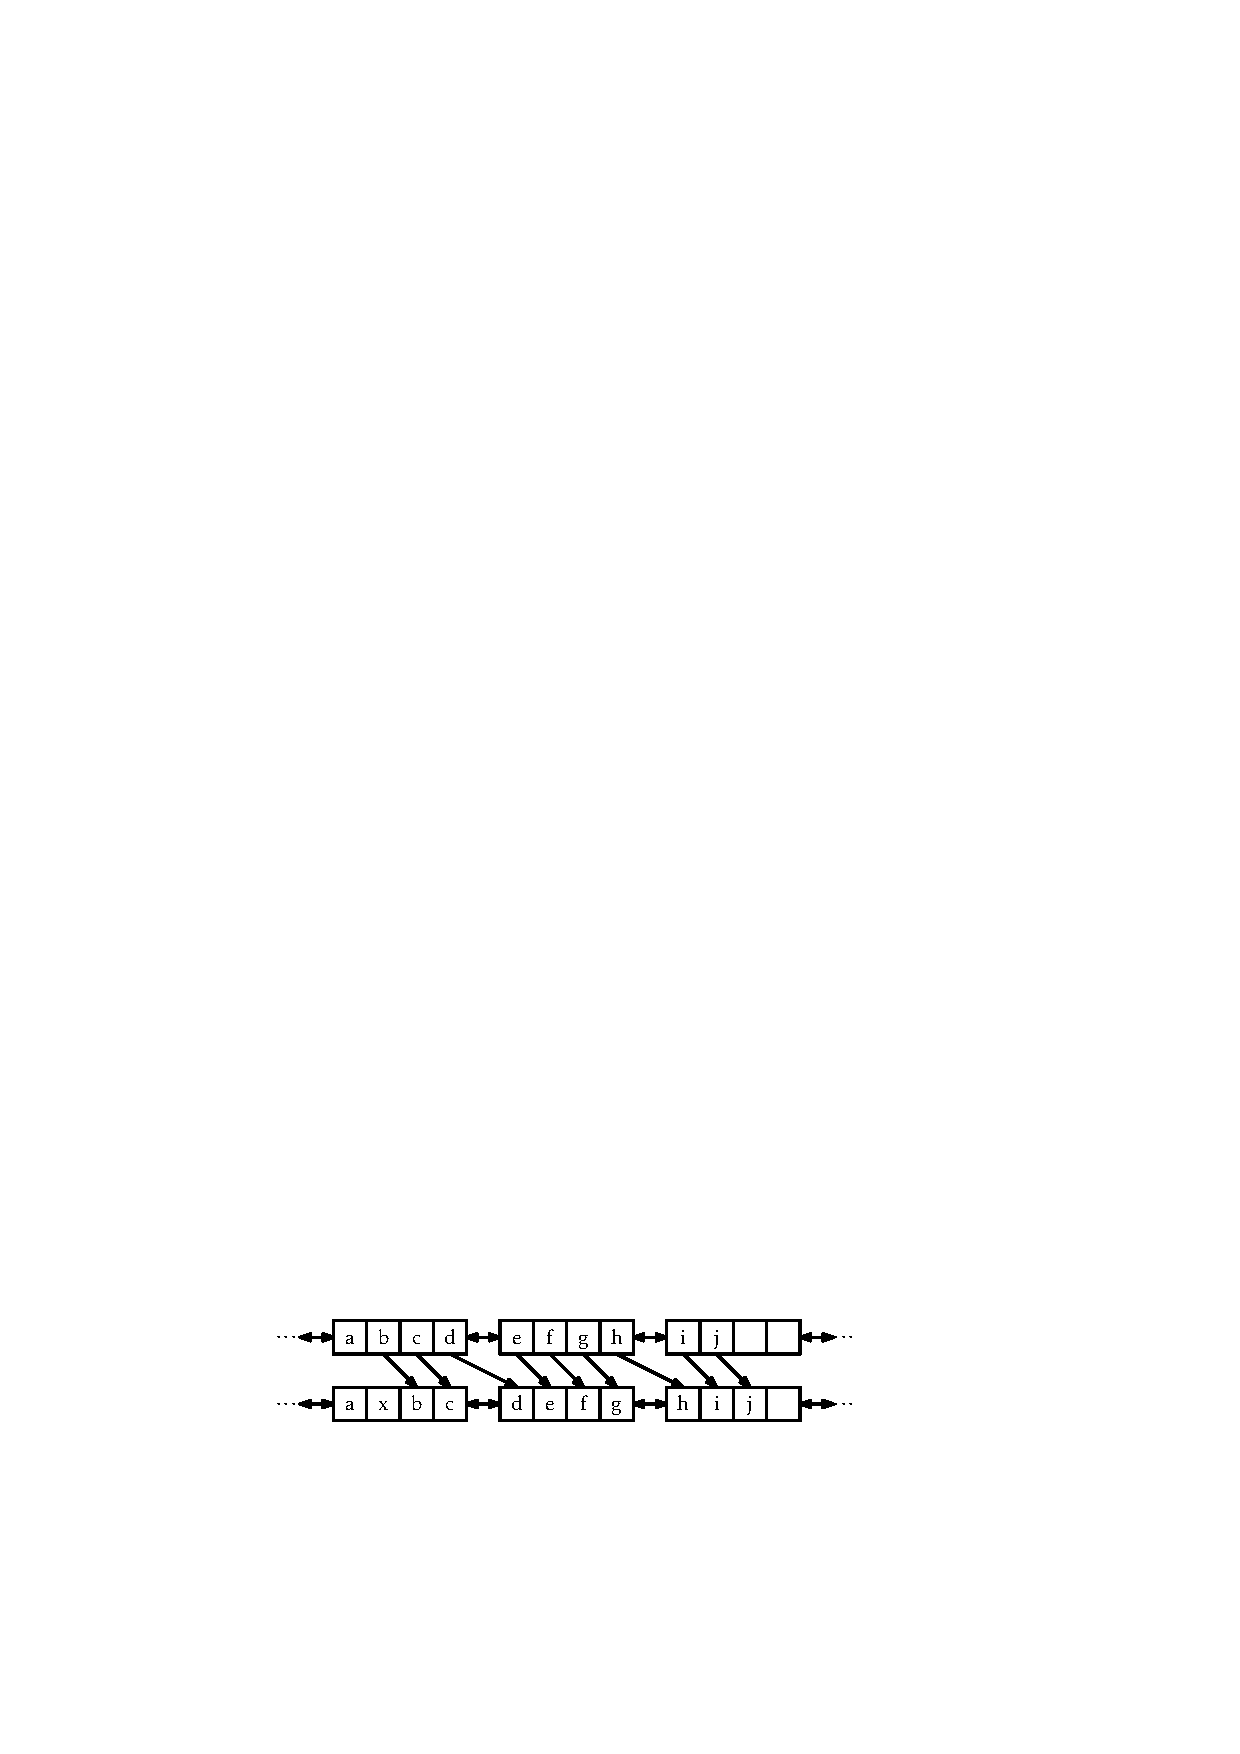
\includegraphics[width=\ScaleIfNeeded]{figs/selist-add-a}\\[4ex]
			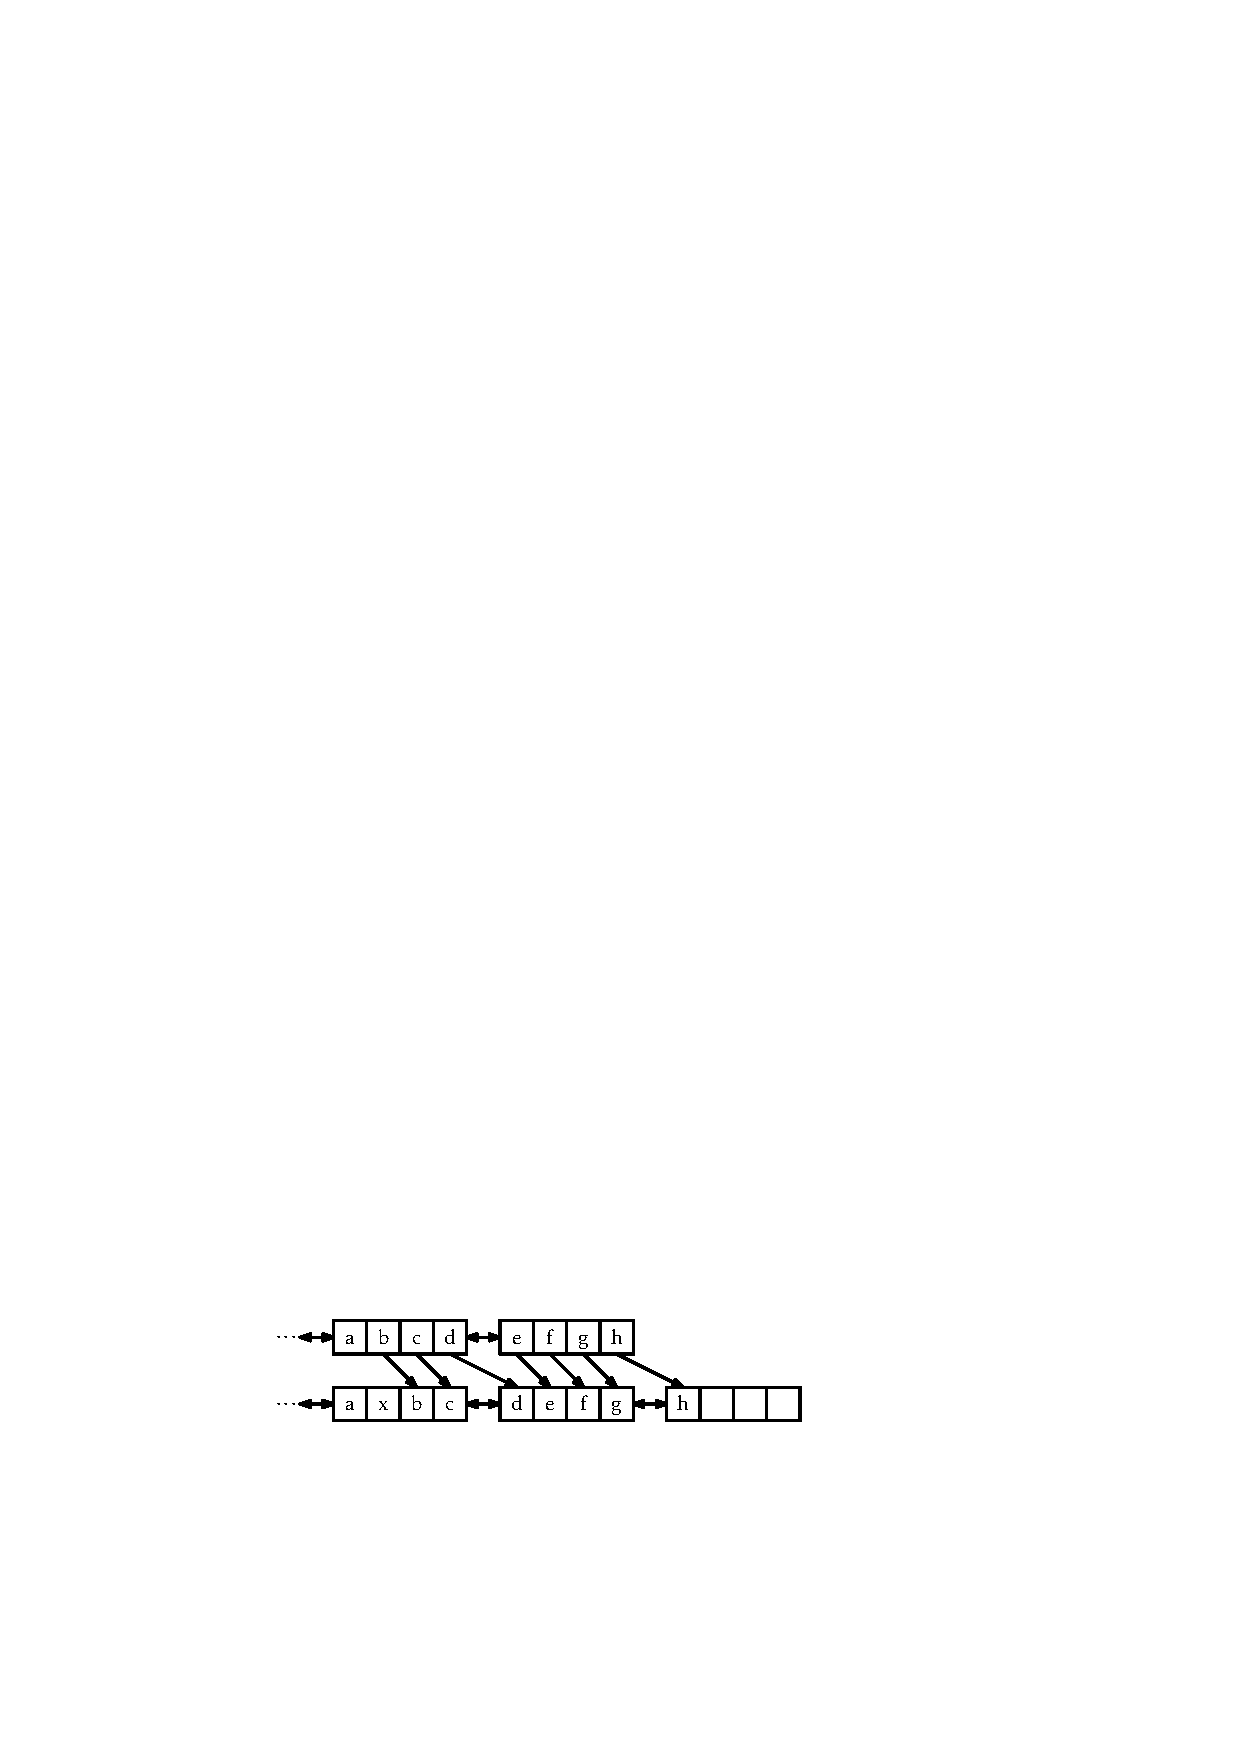
\includegraphics[width=\ScaleIfNeeded]{figs/selist-add-b}\\[4ex]
			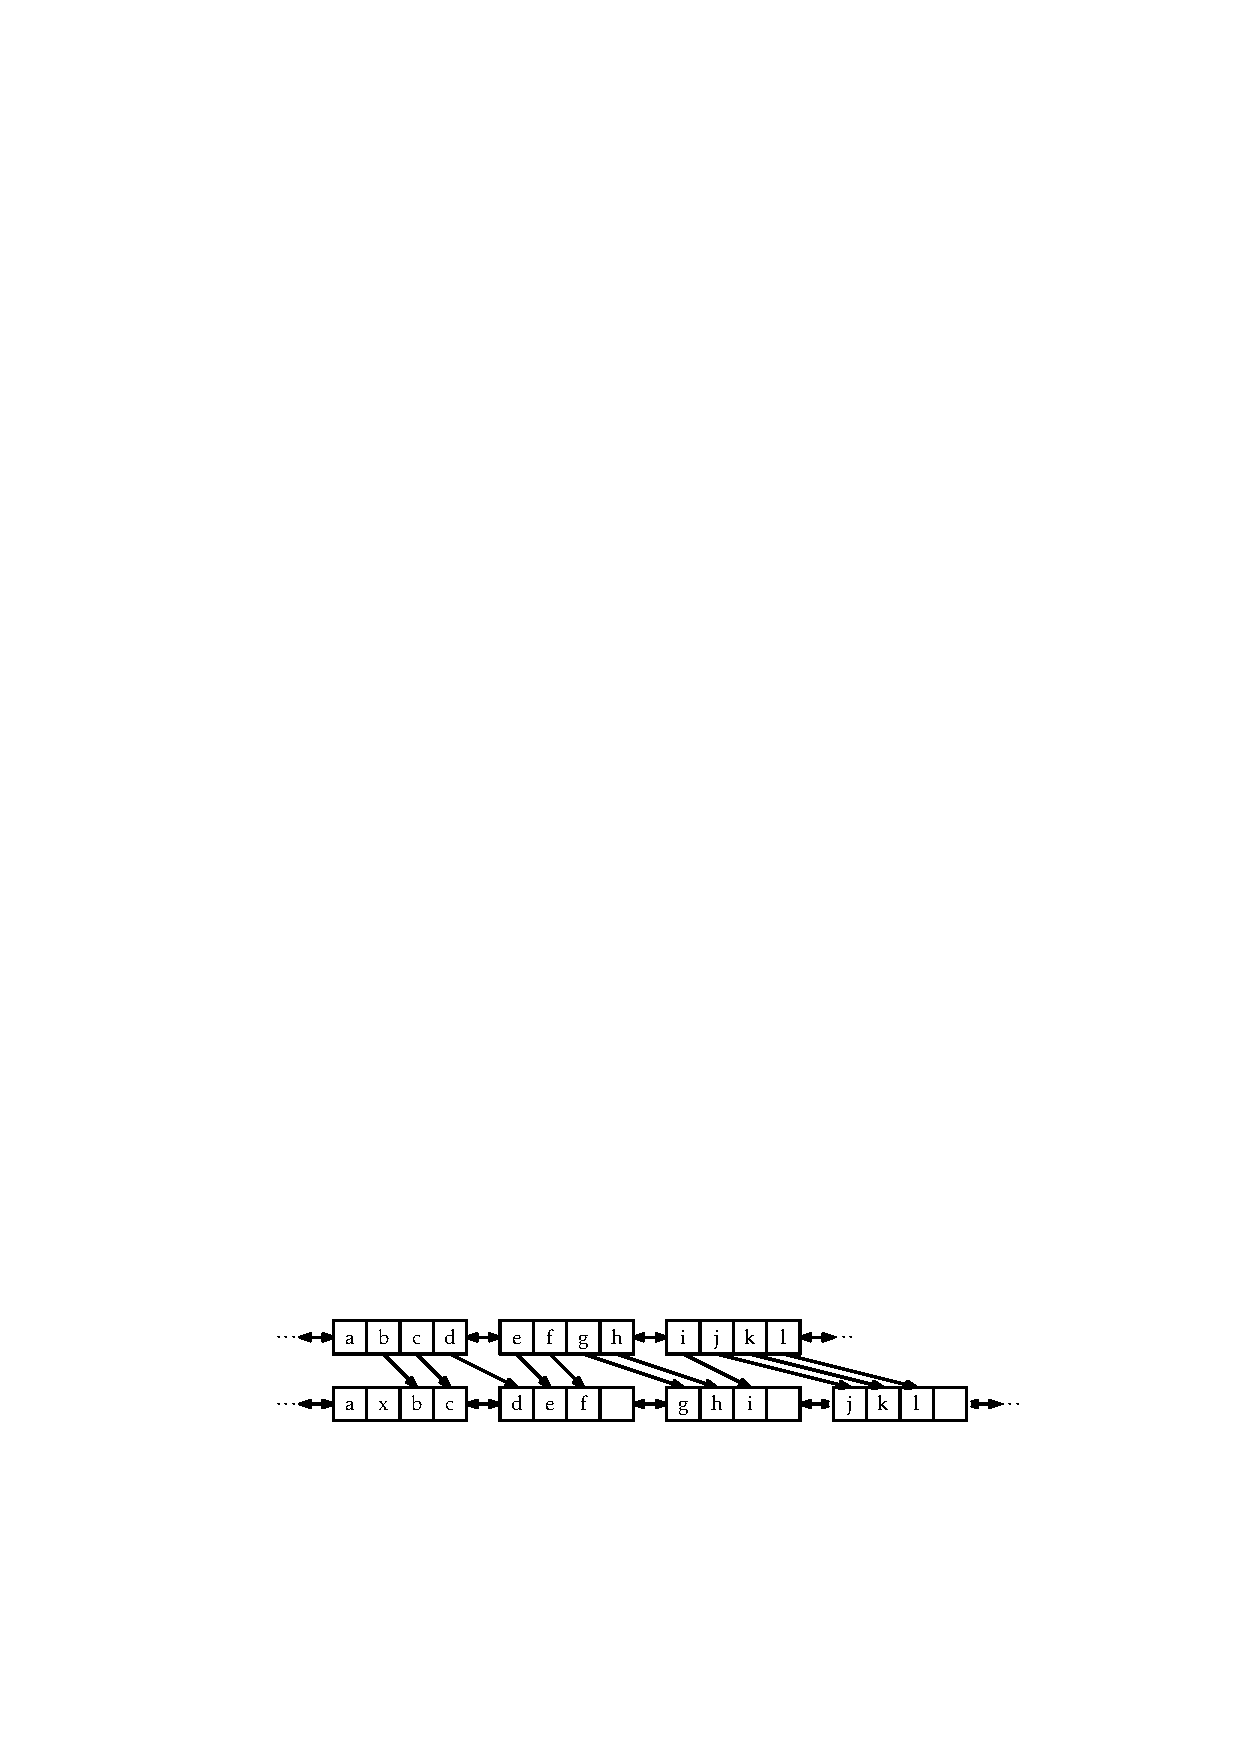
\includegraphics[width=\ScaleIfNeeded]{figs/selist-add-c}\\
		\end{tabular}
	\end{center}
	\caption[SEList add]{Os três casos que ocorrem durante a adição de um item #x# no interior de uma #SEList#.  (Essa #SEList# tem bloco de tamanho $#b#=3$.)}
	\figlabel{selist-add}
\end{figure}
%Fim Lucas

%Inicio Gabriel

\begin{enumerate}
	\item Nós, rapidamente, (em $r+1\le #b#$ passos) achamos um nó $#u#_r$ cujo bloco não está cheio.  Neste caso, executamos $r$ deslocamentos de um elemento de um bloco para o próximo, de modo que um espaço livre em $#u#_r$ se torne um espaço livre em $#u#_0$.  Podemos, então, inserir #x# no bloco $#u#_0$.
	
	\item Nós, rapidamente, (em $r+1\le #b#$ passos) chegamos ao fim da lista
	de blocos.  Neste caso, adicionamos um novo bloco vazio ao final da
	lista de blocos e procedemos como no primeiro caso.
	
	\item Após #b# passos não encontramos nenhum bloco que não está cheio.
	Neste caso, $#u#_0,\ldots,#u#_{#b#-1}$ é uma sequência de blocos #b#,
	em que cada um contém $#b#+1$ elementos. Inserimos um novo bloco $#u#_{#b#}$
	ao final desta sequência e \emph{distribuímos} os $#b#(#b#+1)$
	elementos originais para que cada bloco de $#u#_0,\ldots,#u#_{#b#}$ contenha exatamente
	#b# elementos. Agora, o bloco de $#u#_0$ contém apenas #b# elementos, portanto ele tem
	espaço para inserirmos #x#.
\end{enumerate}

\codeimport{ods/SEList.add(i,x)}

O tempo de execução da operação #add(i,x)# depende que cada um dos
três casos acima ocorra. Os casos~1 e 2 envolvem examinar e 
deslocar elementos através de, no máximo, #b# blocos e demoram $O(#b#)$.
O caso~3 envolve chamar o método #spread(u)#, que  move $#b#(#b#+1)$
elementos e demora $O(#b#^2)$.  Se nós ignorarmos o custo do Caso~3
(o que explicaremos mais adiante com a amortização), isto significa que
o tempo de execução total para localizar #i# e executar a inserção de #x#
é $O(#b#+\min\{#i#,#n#-#i#\}/#b#)$.

\subsection{Remover um Elemento}

Remover um elemento de uma #SEList# é similar a adicionar um elemento.
Primeiro, localizamos o nó #u# que contém o elemento de índice #i#.
Agora, temos que estar preparados para o caso em que não podemos remover um elemento
de #u# sem fazer com que o bloco #u# fique menor que $#b#-1$.

Novamente, deixe $#u#_0,#u#_1,#u#_2,\ldots$ indicar #u#, #u.next#, #u.next.next#,
e assim por diante. Examinamos $#u#_0,#u#_1,#u#_2,\ldots$ para procurar
um nó do qual podemos pegar emprestado um elemento para fazer o tamanho do
bloco $#u#_0$ ser, no mínimo, $#b#-1$.  Há três casos a considerar
(ver \figref{selist-remove}):

\begin{figure}
	\noindent
	\begin{center}
		\begin{tabular}{l}
			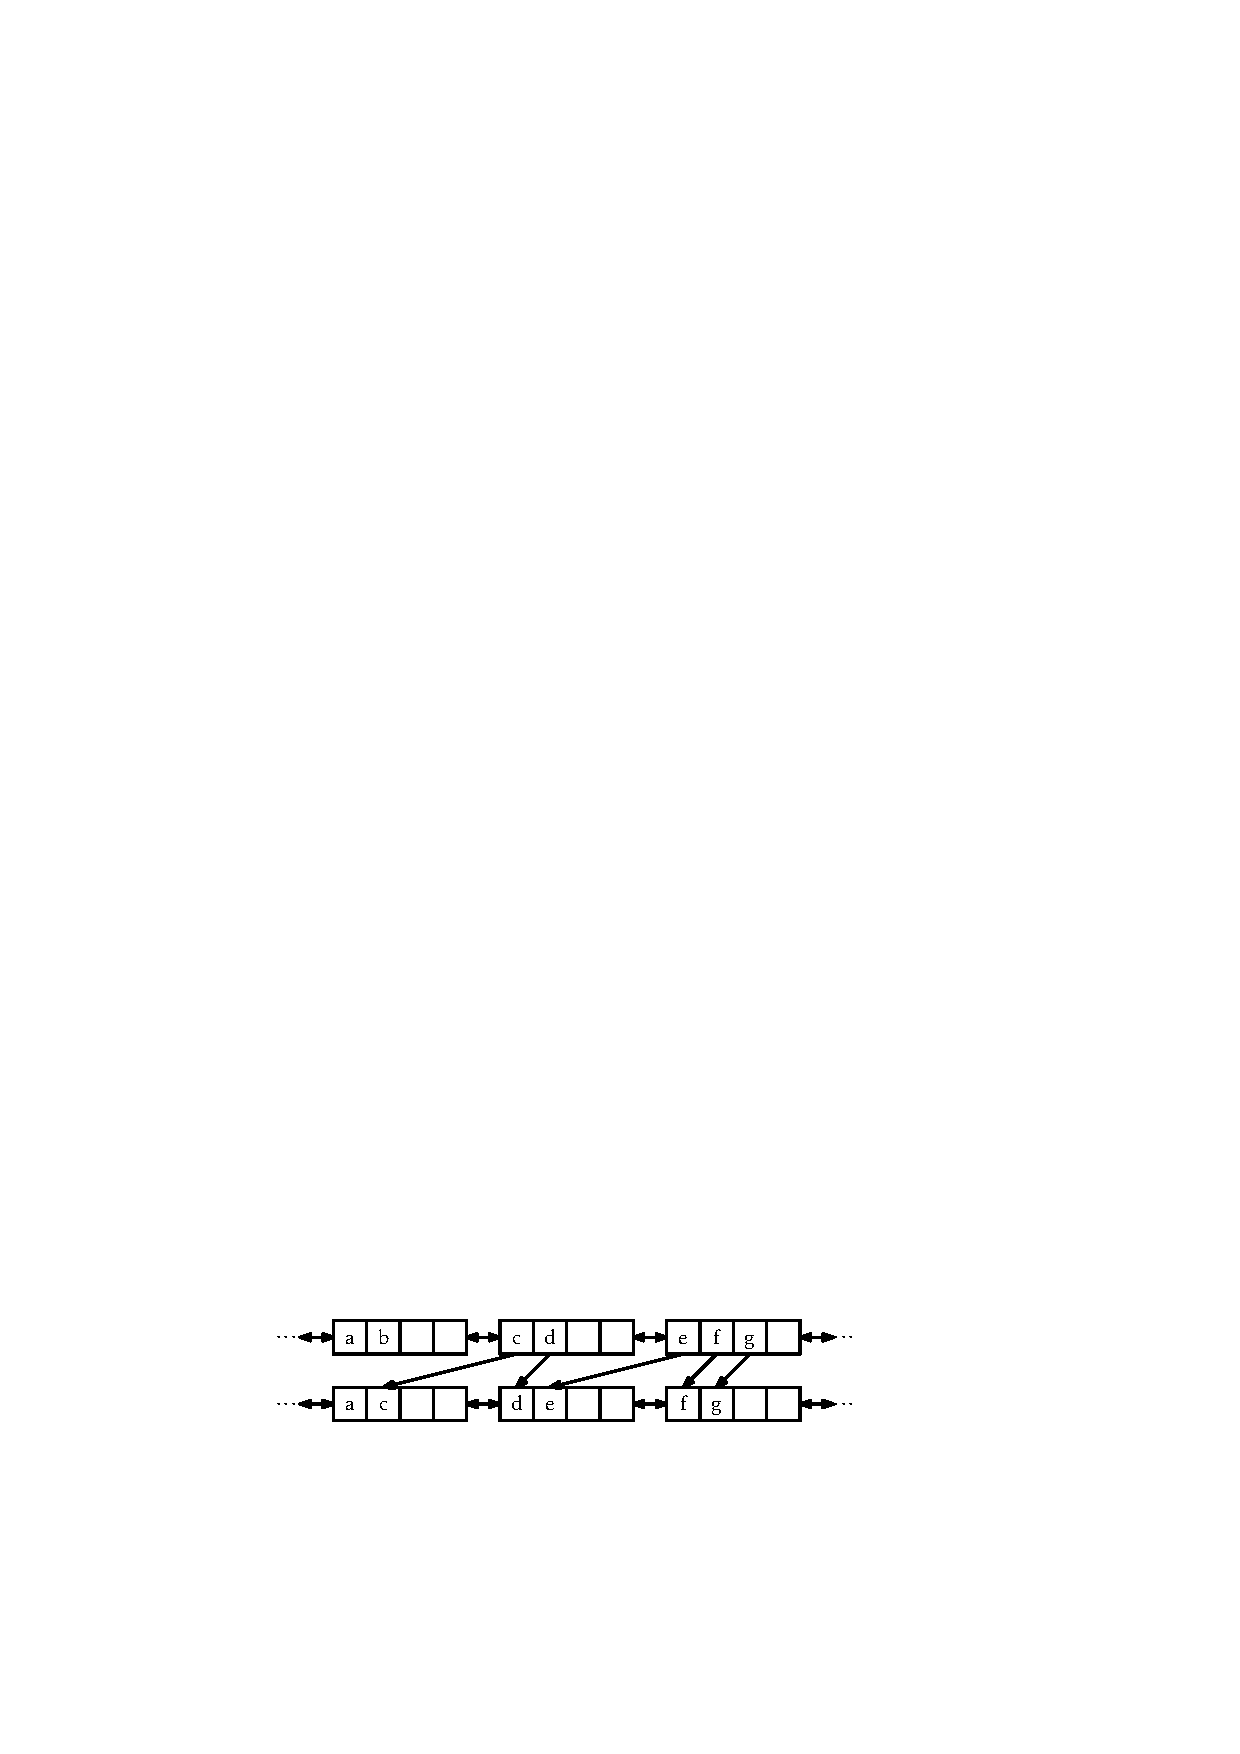
\includegraphics[scale=0.90909]{figs/selist-remove-a}\\[4ex]
			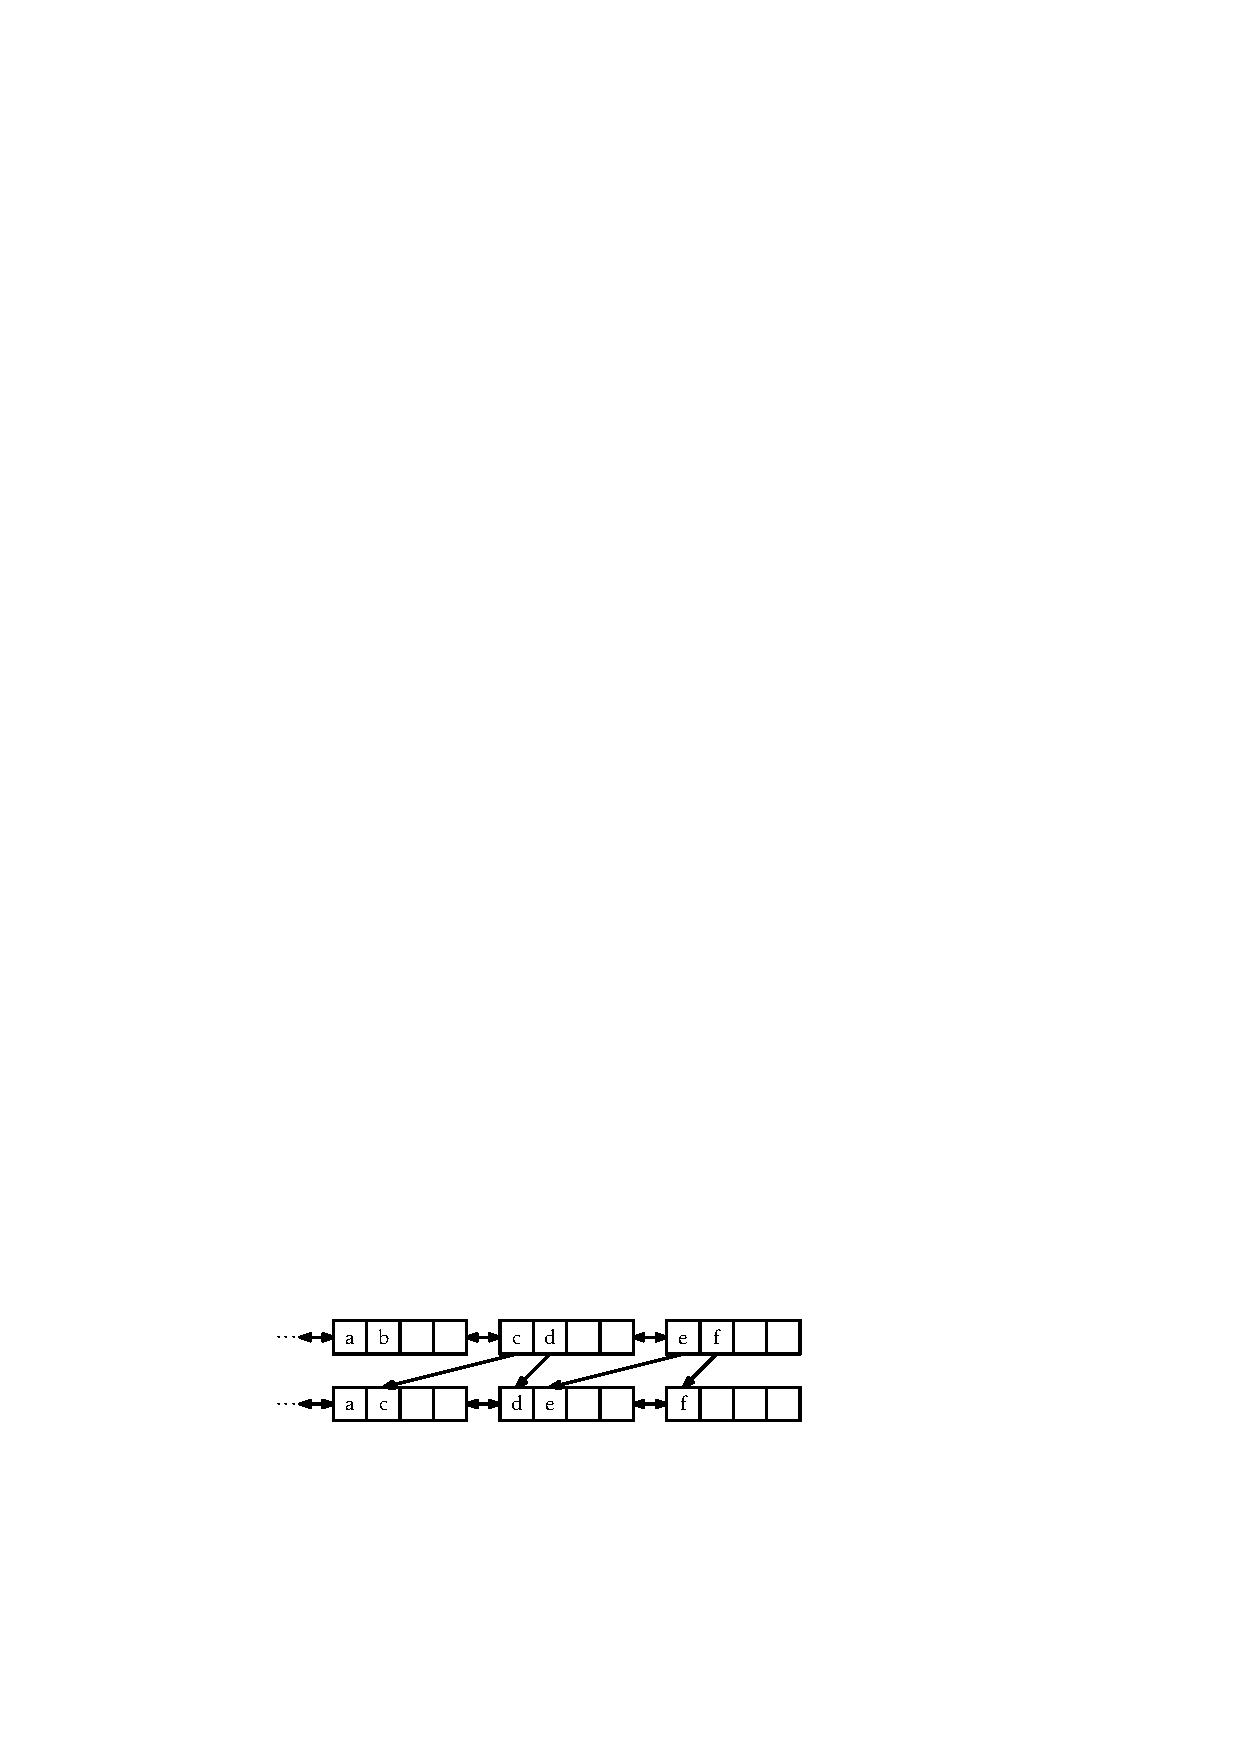
\includegraphics[scale=0.90909]{figs/selist-remove-b}\\[4ex]
			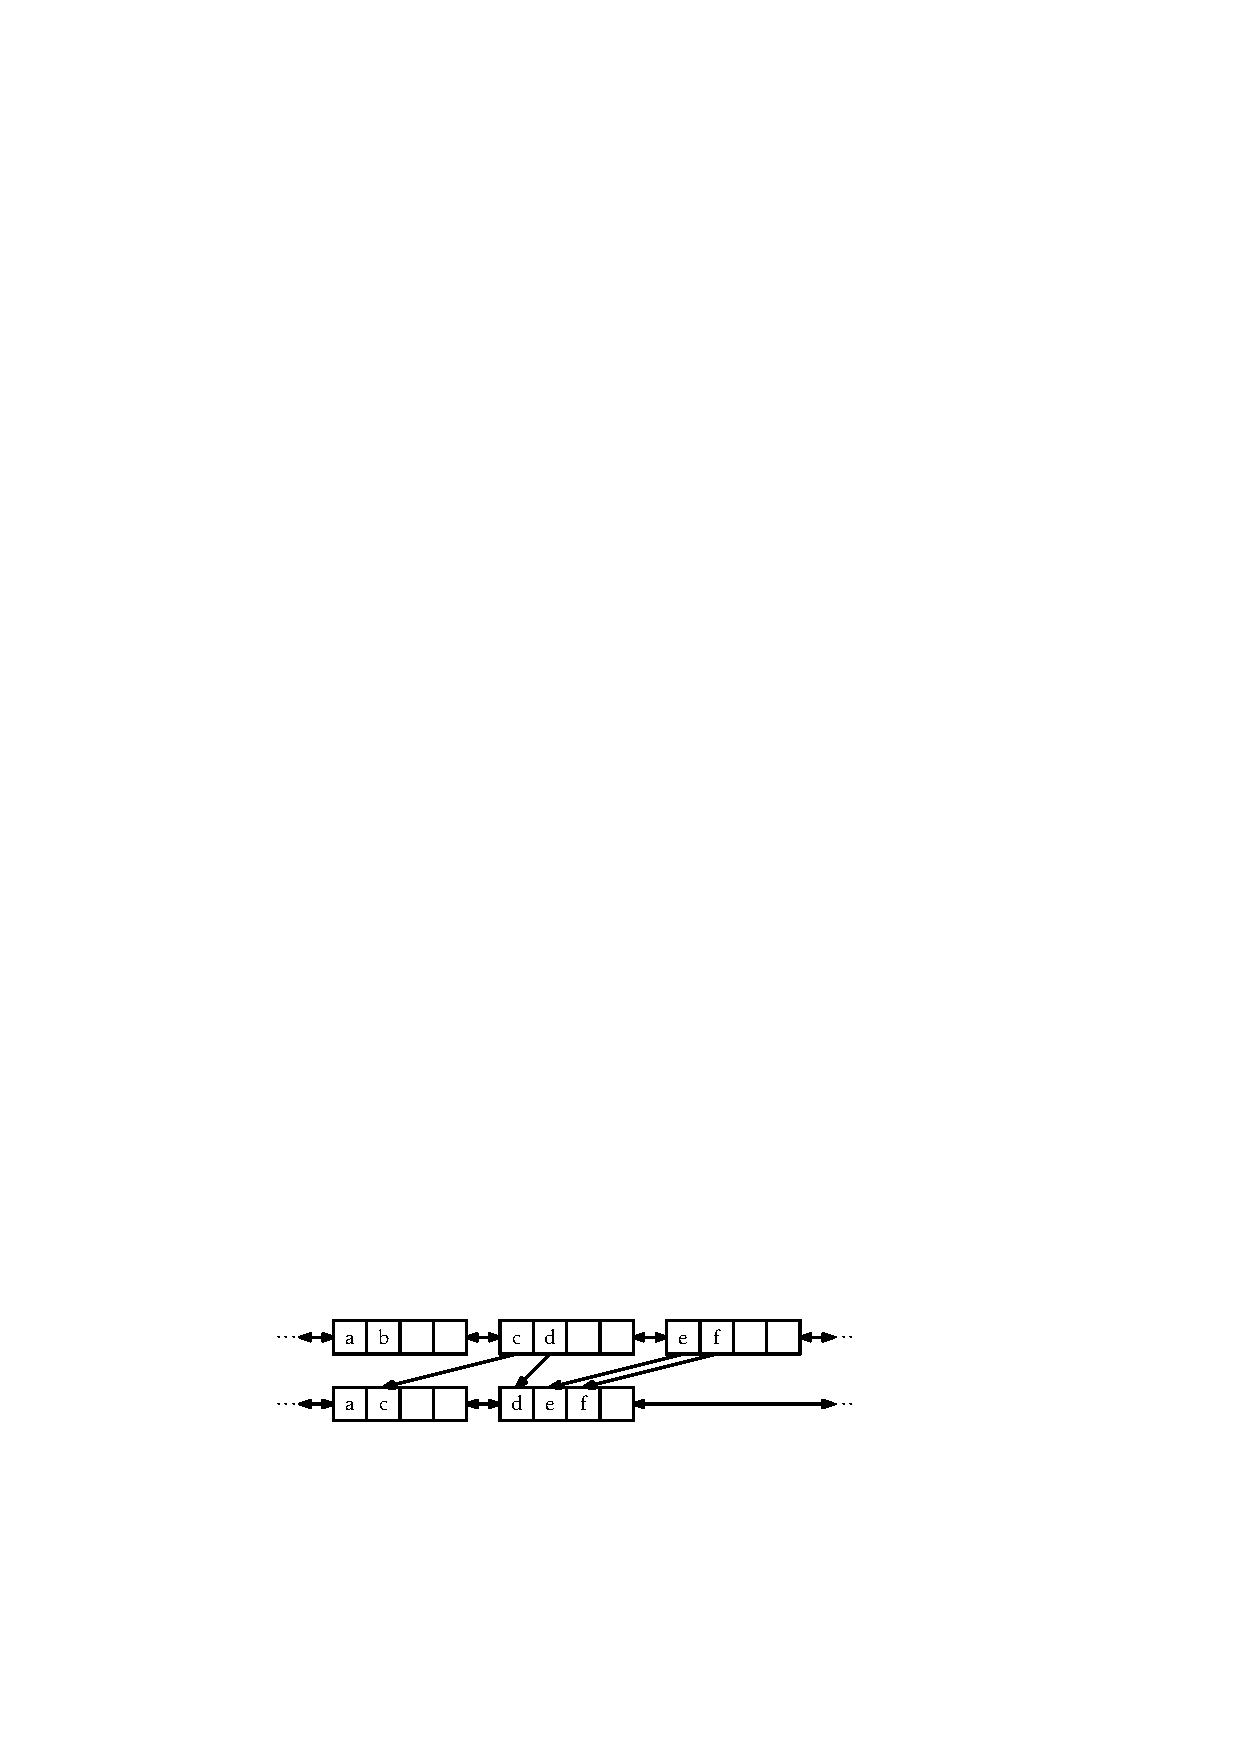
\includegraphics[scale=0.90909]{figs/selist-remove-c}\\
		\end{tabular}
	\end{center}
	\caption[SEList remove]{Os três casos que ocorrem durante a remoção de um item #x# no interior de uma #SEList#.  (Esta #SEList# tem bloco de tamanho $#b#=3$.)}
	\figlabel{selist-remove}
\end{figure}


\begin{enumerate}
	\item Nós, rapidamente, (em $r+1\le #b#$ passos) achamos um nó cujo bloco contém
	mais de $#b#-1$ elementos. Neste caso, executamos $r$ deslocamentos de um
	elemento de um bloco para o anterior, de modo que o elemento extra
	em $#u#_r$ se torne um elemento extra em $#u#_0$. Podemos, então,remover o
	elemento apropriado do bloco $#u#_0$.
	
	\item Nós, rapidamente, (em $r+1\le #b#$ passos) chegamos ao fim da lista de
	blocos. Neste caso, $#u#_r$ é o último bloco, e não há razão 
	para o bloco $#u#_r$ conter, no mínimo, $#b#-1$ elementos.  Portanto,
	procedemos como acima, pegando emprestado um elemento de $#u#_r$ para fazer um elemento
	extra em $#u#_0$.  Se isto fizer com que o bloco $#u#_r$ fique vazio,
	então removemos ele.
	
	\item Após #b# passos, não encontramos nenhum bloco contendo mais de
	$#b#-1$ elementos.  Neste caso, $#u#_0,\ldots,#u#_{#b#-1}$ é uma sequência
	de #b# blocos, em que cada um contém $#b#-1$ elementos. Nós \emph{concentramos}
	estes $#b#(#b#-1)$ elementos em $#u#_0,\ldots,#u#_{#b#-2}$ de modo que cada um
	destes $#b#-1$ blocos contenha exatamente #b# elementos e removemos
	$#u#_{#b#-1}$, que agora está vazio.  Agora, o bloco de $#u#_0$ contém #b#
	elementos e, então, podemos remover o elemento apropriado dele.
\end{enumerate}

\codeimport{ods/SEList.remove(i)}

Como a operação #add(i,x)#, o tempo de execução da operação #remove(i)#
é $O(#b#+\min\{#i#,#n#-#i#\}/#b#)$ se ignorarmos o custo do
método #gather(u)# que ocorre no Caso~3.

\subsection{Análise Amortizada de Distribuição e Concentração}

Em seguida, consideramos o custo dos métodos #gather(u)# e #spread(u)#
que podem ser executados pelos métodos #add(i,x)# e #remove(i)#. Por uma
questão de completude, aqui estão:

\codeimport{ods/SEList.spread(u)}
\codeimport{ods/SEList.gather(u)}
%Fim Gabriel

%Inicio Ester
O tempo de execução de cada um destes métodos é dominado pelos dois
loops aninhados. Ambos os loops, internos e externos, executam no máximo
$#b#+1$ vezes, de modo que o tempo de execução total de cada um destes métodos
é $O((#b#+1)^2)=O(#b#^2)$. No entanto, o seguinte lema mostra que
estes métodos executam no máximo um de cada #b# chamadas para #add(i,x)#
ou #remove(i)#.

\begin{lem}\lemlabel{selist-amortized}
	Se for criado uma #SEList# vazia e qualquer sequência de $m\ge 1$ chamadas
	para #add(i,x)# e #remove(i)# for executado, então o tempo total
	gasto durante as chamadas para #spread()# e #gather()# é $O(#b#m)$.
\end{lem}

\begin{proof}
	Nós usaremos o método potencial de análise amortizada.
	\index{Método potencial}%
	Dizemos que
	um nó #u# é \emph{frágil} se o bloco #u# não contém #b#
	elementos (de modo que #u# seja o último nó, ou contenha $#b#-1$
	ou $#b#+1$ elementos).  Qualquer nó cujo bloco contenha #b# elementos é
	\emph{rígido}. Defina o \emph{potential} de uma #SEList# como o número
	de nós frágeis que contém.  Consideramos apenas a operação
	#add(i,x)# e sua relação com o número de chamadas para #spread(u)#.
	A análise de #remove(i)# e #gather(u)# é idêntica.
	
	Observe que, se o Caso~1 ocorrer durante o método #add(i,x)#, então
	somente um nó, $#u#_r$, tem o tamanho de seu bloco alterado. Portanto,
	no máximo um nó, ou seja $#u#_r$, irá de rígido a frágil.
	Se ocorrer o Caso~2, então um novo nó é criado, e este novo nó
	será frágil, mas nenhum outro nó mudará de tamanho, então o número de nós
	frágeis aumentará em um.  Assim, tanto no Caso~1 ou no Caso~2 o potencial
	do SEList aumentará para no máximo um.
	
	Finalmente, se ocorre o Caso~3, é porque $#u#_0,\ldots,#u#_{#b#-1}$
	são todos nós frágeis.  Então $#spread(#u_0#)#$ é chamado e estes #b#
	nós frágeis são substituídos por $#b#+1$ nós rígidos.  Finalmente, #x#
	é adicionado ao bloco $#u#_0$, fazendo $#u#_0$ frágil.  No total, o
	potencial diminui em $#b#-1$.
	
	Em resumo, o potencial começa em 0 (não há nós na lista).
	Cada vez que Caso~1 ou Caso~2 ocorre, o potencial aumenta, em no
	máximo, 1.  Cada vez que ocorre o Caso~3, o potencial diminui para $#b#-1$.
	O potencial (que conta o número de nós frágeis) nunca é menor
	que 0.  Nós concluímos que, para cada ocorrência do Caso~3, há
	pelo menos $#b#-1$ ocorrências do Caso~1 ou Caso~2.  Assim, para cada
	chamada para #spread(u)# existem pelo menos #b# chamadas para #add(i,x)#.
	Isso completa a verificação.
\end{proof}

\subsection{Resumo}

O seguinte teorema resume o desempenho das estruturas de dados de #SEList#:

\begin{thm}\thmlabel{selist}
	Um #SEList# implementa a interface de #Lista#.  Ignorando o custo das
	chamadas para #spread(u)# e #gather(u)#, uma #SEList# com tamanho de bloco #b#
	supporta as operações
	\begin{itemize}
		\item #get(i)# e #set(i,x)# em $O(1+\min\{#i#,#n#-#i#\}/#b#)$ vezes por operação; e
		\item #add(i,x)# e #remove(i)# em $O(#b#+\min\{#i#,#n#-#i#\}/#b#)$ vezes por operação.
	\end{itemize}
	Além disso, começando com uma #SEList# vazia, qualquer sequência de operações 
	$m$ #add(i,x)# e #remove(i)# resulta em um tempo total gasto de $O(#b#m)$
	  durante todas as chamadas para #spread(u)# e #gather(u)#.
	
	O espaço (medido em palavras)\footnote{Releia a \secref{model} para uma discussão
		de como a memória é medida.} usado por uma #SEList#
	que armazena #n# elementos é $#n# +O(#b# + #n#/#b#)$.
\end{thm}

A #SEList# é um compromisso entre uma #ArrayList# e uma #DLList# na qual
a mistura relativa destas duas estruturas depende do tamanho do bloco #b#.
No extremo $#b#=2$, cada #SEList# armazena no máximo três valores,
o que não é muito diferente da #DLList#. No outro extremo,
$#b#>#n#$, todos os elementos são armazenados em um único array, assim como em
um #ArrayList#.  Entre esses dois extremos reside uma troca entre
o tempo que leva para adicionar ou remover um item da lista e o tempo que leva para
localizar um item de lista particular.

\section{Discussão e Exercícios}

Tanto as listas simplesmente encadeadas e as listas duplamente encadeadas são técnicas estabelecidas,
tendo sido utilizadas em programas há mais de 40 anos.  Elas são discutidas,
por exemplo, por Knuth \cite[Seções~2.2.3--2.2.5]{k97v1}.  Mesmo a
estrutura de dados #SEList# parece ser um exercício bem conhecido de estruturas de dados.
A #SEList# é as vezes chamada de \emph{unrolled linked list}
\cite{sra94}.
\index{unrolled linked list|seealso{#SEList#}}%
\index{linked list!unrolled|seealso{#SEList#}}%

Outra maneira de economizar espaço em uma lista duplamente encadeada é usar as chamadas
listas XOR.
\index{XOR-list}%
Em uma lista XOR, cada nó, #u#, contém apenas um
ponteiro, chamado #u.nextprev#, que contém o \textit{ou exclusivo bi-a-bit} de #u.prev#
e #u.next#.  A própria lista precisa armazenar dois ponteiros, um para o nó #dummy#
e um para #dummy.next# (o primeiro nó, ou #dummy# se a lista estiver
vazia). Esta técnica utiliza o fato de que, se temos um ponteiro para #u#
e #u.prev#, então podemos extrair #u.next# usando a fórmula
\[
#u.next# = #u.prev# \verb+^+ #u.nextprev# \enspace .
\]
%Fim Ester

%Inicio Diana
(Here \verb+^+ computes the bitwise exclusive-or of its two arguments.)
This technique complicates the code a little and is not possible in
some languages, like Java and Python, that have garbage collection but gives a
doubly-linked list implementation that requires only one pointer per node.
See Sinha's magazine article \cite{s04} for a detailed discussion of
XOR-lists.

\begin{exc}
  Why is it not possible to use a dummy node in an #SLList# to avoid
  all the special cases that occur in the operations #push(x)#, #pop()#,
  #add(x)#, and #remove()#?
\end{exc}

\begin{exc}
  Design and implement an #SLList# method, #secondLast()#, that returns
  the second-last element of an #SLList#.  Do this without using the
  member variable, #n#, that keeps track of the size of the list.
\end{exc}

\begin{exc}
  Implement the #List# operations #get(i)#, #set(i,x)#,
  #add(i,x)# and #remove(i)# on an #SLList#.  Each of these operations
  should run in $O(1+#i#)$ time.
\end{exc}

\begin{exc}
  Design and implement an #SLList# method, #reverse()# that reverses the
  order of elements in an #SLList#.  This method should run in $O(#n#)$
  time, should not use recursion, should not use any secondary data
  structures, and should not create any new nodes.
\end{exc}

\begin{exc}
  Design and implement #SLList# and #DLList# methods called #checkSize()#.
  These methods walk through the list and count the number of nodes to
  see if this matches the value, #n#, stored in the list.  These methods
  return nothing, but throw an exception if the size they compute does
  not match the value of #n#.
\end{exc}

\begin{exc}
  Try to recreate the code for the #addBefore(w)# operation that creates a
  node, #u#, and adds it in a #DLList# just before the node #w#.  Do not
  refer to this chapter.  Even if your code does not exactly match the
  code given in this book it may still be correct.  Test it and see if
  it works.
\end{exc}

The next few exercises involve performing manipulations on #DLList#s.
You should complete them without allocating any new nodes or temporary
arrays.  They can all be done only by changing the #prev# and #next#
values of existing nodes.

\begin{exc}
  Write a #DLList# method #isPalindrome()# that returns #true# if the
  list is a \emph{palindrome},
  \index{palindrome}%
  i.e., the element at position #i# is equal to
  the element at position $#n#-i-1$ for all $i\in\{0,\ldots,#n#-1\}$.
  Your code should run in $O(#n#)$ time.
\end{exc}

\begin{exc}
  Implement a method #rotate(r)# that ``rotates'' a #DLList# so that list
  item #i# becomes list item $(#i#+#r#)\bmod #n#$.  This method should
  run in $O(1+\min\{#r#,#n#-#r#\})$ time and should not modify any nodes in
  the list.
\end{exc}


\begin{exc}\exclabel{linkedlist-truncate}
  Write a method, #truncate(i)#, that truncates a #DLList# at position
  #i#.  After executing this method, the size of the list will be #i# and
  it should contain only the elements at indices $0,\ldots,#i#-1$.  The
  return value is another #DLList# that contains the elements at indices
  $#i#,\ldots,#n#-1$.  This method should run in $O(\min\{#i#,#n#-#i#\})$
  time.
\end{exc}

\begin{exc}
  Write a #DLList# method, #absorb(l2)#, that takes as an argument
  a #DLList#, #l2#, empties it and appends its contents, in order,
  to the receiver.  For example, if #l1# contains $a,b,c$ and #l2#
  contains $d,e,f$, then after calling #l1.absorb(l2)#, #l1# will contain
  $a,b,c,d,e,f$ and #l2# will be empty.
\end{exc}

\begin{exc}
  Write a method #deal()# that removes all the elements with odd-numbered
  indices from a #DLList# and return a #DLList# containing these elements.
  For example, if #l1#, contains the elements $a,b,c,d,e,f$, then after
  calling #l1.deal()#, #l1# should contain $a,c,e$ and a list containing
  $b,d,f$ should be returned.
\end{exc}
%Fim Diana

%Daniel
\begin{exc}
	Escreva um método, #reverse()#, que inverta a ordem dos elementos em
	uma #DLList#.  
\end{exc}

\begin{exc}\exclabel{dllist-sort}
	\index{merge-sort}%
	Este exercício orienta você através de uma implementação do algoritimo
	merge-sort para classificar uma #DLList#, como discutido na \secref{merge-sort}.
	\javaonly{Em sua implementação, faça comparações entre elementos
		usando o método de #compareTo(x)# de modo que a implementação resultante possa
		classificar qualquer #DLList# contendo elementos que implementam a interface #Comparable#.}
	\begin{enumerate}
		\item Escreva o método #DLList# chamado #takeFirst(l2)#.
		Este método leva o primeiro nó de #l2# e adiciona-o à
		lista de recepção.  Isso equivale a #add(size(),l2.remove(0))#,
		exceto que ele não deve criar um novo nó.
		\item Escreva um método estático de #DLList#, #merge(l1,l2)#, que recebe duas
		listas classificadas #l1# e #l2#, mescla-as e retorna uma nova
		lista contendo o resultado.  Isso tem como consequência que #l1# e #l2# se tornam vazias
		no processo.  Por exemplo, se #l1# contém $a,c,d$ e #l2# contém
		$b,e,f$, assim este método retorna uma nova lista contendo $a,b,c,d,e,f$.
		\item Escreva um método #DLList#  #sort()# que classifica os elementos
		contidos na lista usando o algoritmo de ordenação por mesclagem.
		Este algoritmo recursivo funciona da seguinte maneira :
		\begin{enumerate}
			\item Se a lista contém 0 ou 1 elementos, então
			não há nada a fazer. Caso contrário,
			\item Usando o método #truncate(size()/2)#, divide a lista
			em duas listas de comprimento aproximadamente igual, #l1# e #l2#;
			\item Recursivamente classificar #l1#;
			\item Recursivamente classificar #l2#; e, finalmente,
			\item  Mesclar #l1# e #l2# em uma única lista ordenada.
		\end{enumerate}
	\end{enumerate}
\end{exc}


Os próximos exercícios são mais avançados e requerem uma
compreensão do que acontece com o valor mínimo armazenado em uma #Stack#
ou #Queue#  à medida que os itens são adicionados e removidos.

\begin{exc}
	\index{MinStack@#MinStack#}%
	Projetar e implementar uma estrutura de dados #MinStack# que pode armazenar
	elementos comparáveis e suporta as operações de pilha #push(x)#,
	#pop()#, e #size()#, assim como a operação de #min()#, que
	retorna o valor mínimo atualmente armazenado na estrutura de dados.
	Todas as operações devem ser executadas em tempo constante.
\end{exc}

\begin{exc}
	\index{MinQueue@#MinQueue#}%
	Projetar e implementar uma estrutura de dados #MinQueue# que pode armazenar
	elementos comparáveis e suporta as operações de fila #add(x)#,
	#remove()#, e #size()#, assim como a operação de #min()#, que
	retorna o valor mínimo atualmente armazenado na estrutura de dados.
	Todas as operações devem ser executadas em tempo constante.
\end{exc}

\begin{exc}
	\index{MinDeque@#MinDeque#}%
	Projetar e implementar a #MinDeque# uma estrutura de dados que pode armazenar
	elementos comparáveis e suporta todas as operações de deque #addFirst(x)#,
	#addLast(x)# #removeFirst()#, #removeLast()# e #size()#,e a 
	operação #min()#, que retorna o menor valor atualmente armazenado em
	estrutura de dados.  Todas as operações devem ser executadas em tempo 
	constante.
\end{exc}

Os próximos exercícios são projetados para testar o entendimento do leitor 
da implementação e análise da lista eficiente em espaço #SEList#:

\begin{exc}
	Prove que, se uma #SEList# é usada como uma #Stack# (para que as
	únicas modificações no #SEList# sejam feitas usando $#push(x)#\equiv
	#add(size(),x)#$ e $#pop()#\equiv #remove(size()-1)#$), então esta
	operação executado em tempo amortizado constante, independente do valor
	de #b#.
\end{exc}

\begin{exc}
	Projetar e implementar uma versão de um #SEList# que suporte todas as
	operações #Deque# em tempo amortizado constante por operação,
	independente do valor de #b#.
\end{exc}

\begin{exc}
	Explicar como usar o operador exclusivo de bit ou operador, \verb+^+, para
	trocar os valores de duas variáveis #int# sem usar uma terceira variável.
\end{exc}
%Fim Daniel



